One requirment of our assignment was to review the clustering accuracy of the fuzzy c-means algorithm as applied to the skewed MNIST dataset.
The fuzzy c-means algorithm is a clustering algorithm that is based on the minimization of the objective function. 
The objective function is a function that is used to measure the quality of a clustering. The objective function was defined above in equation~\ref{eq:objective_function}.
When clustering is finished we need to compare the clusters that were produced to the actual labels of the data. We will use the rand index to compare the clusters to the labels. The rand index is defined as follows:
\begin{equation}
\label{eq:rand_index}
RI = \frac{n_{00} + n_{11}}{n_{00} + n_{11} +n_{01} + n_{10}} = \frac{n_{00} + n_{11}}{{n \choose 2}}
\end{equation}
where $n_{11}$ is the number of pairs of elements that are in the same cluster and in the same class, $n_{00}$ is the number of pairs of elements that are in different clusters and in different classes, and ${n} \choose {2}$ is the total number of pairs of elements in the dataset. 
The rand index is a value between 0 and 1. 
A value of 1 indicates that the clusters are identical to the labels.
A value of 0 indicates that the clusters are completely different from the labels. 
The rand index is a good measure of the accuracy of the clustering algorithm. 

While the FCM algorithm was running, we decided to review the progression of J, eq.~\ref{eq:objective_function}.

\begin{figure}[H]
    \centering
    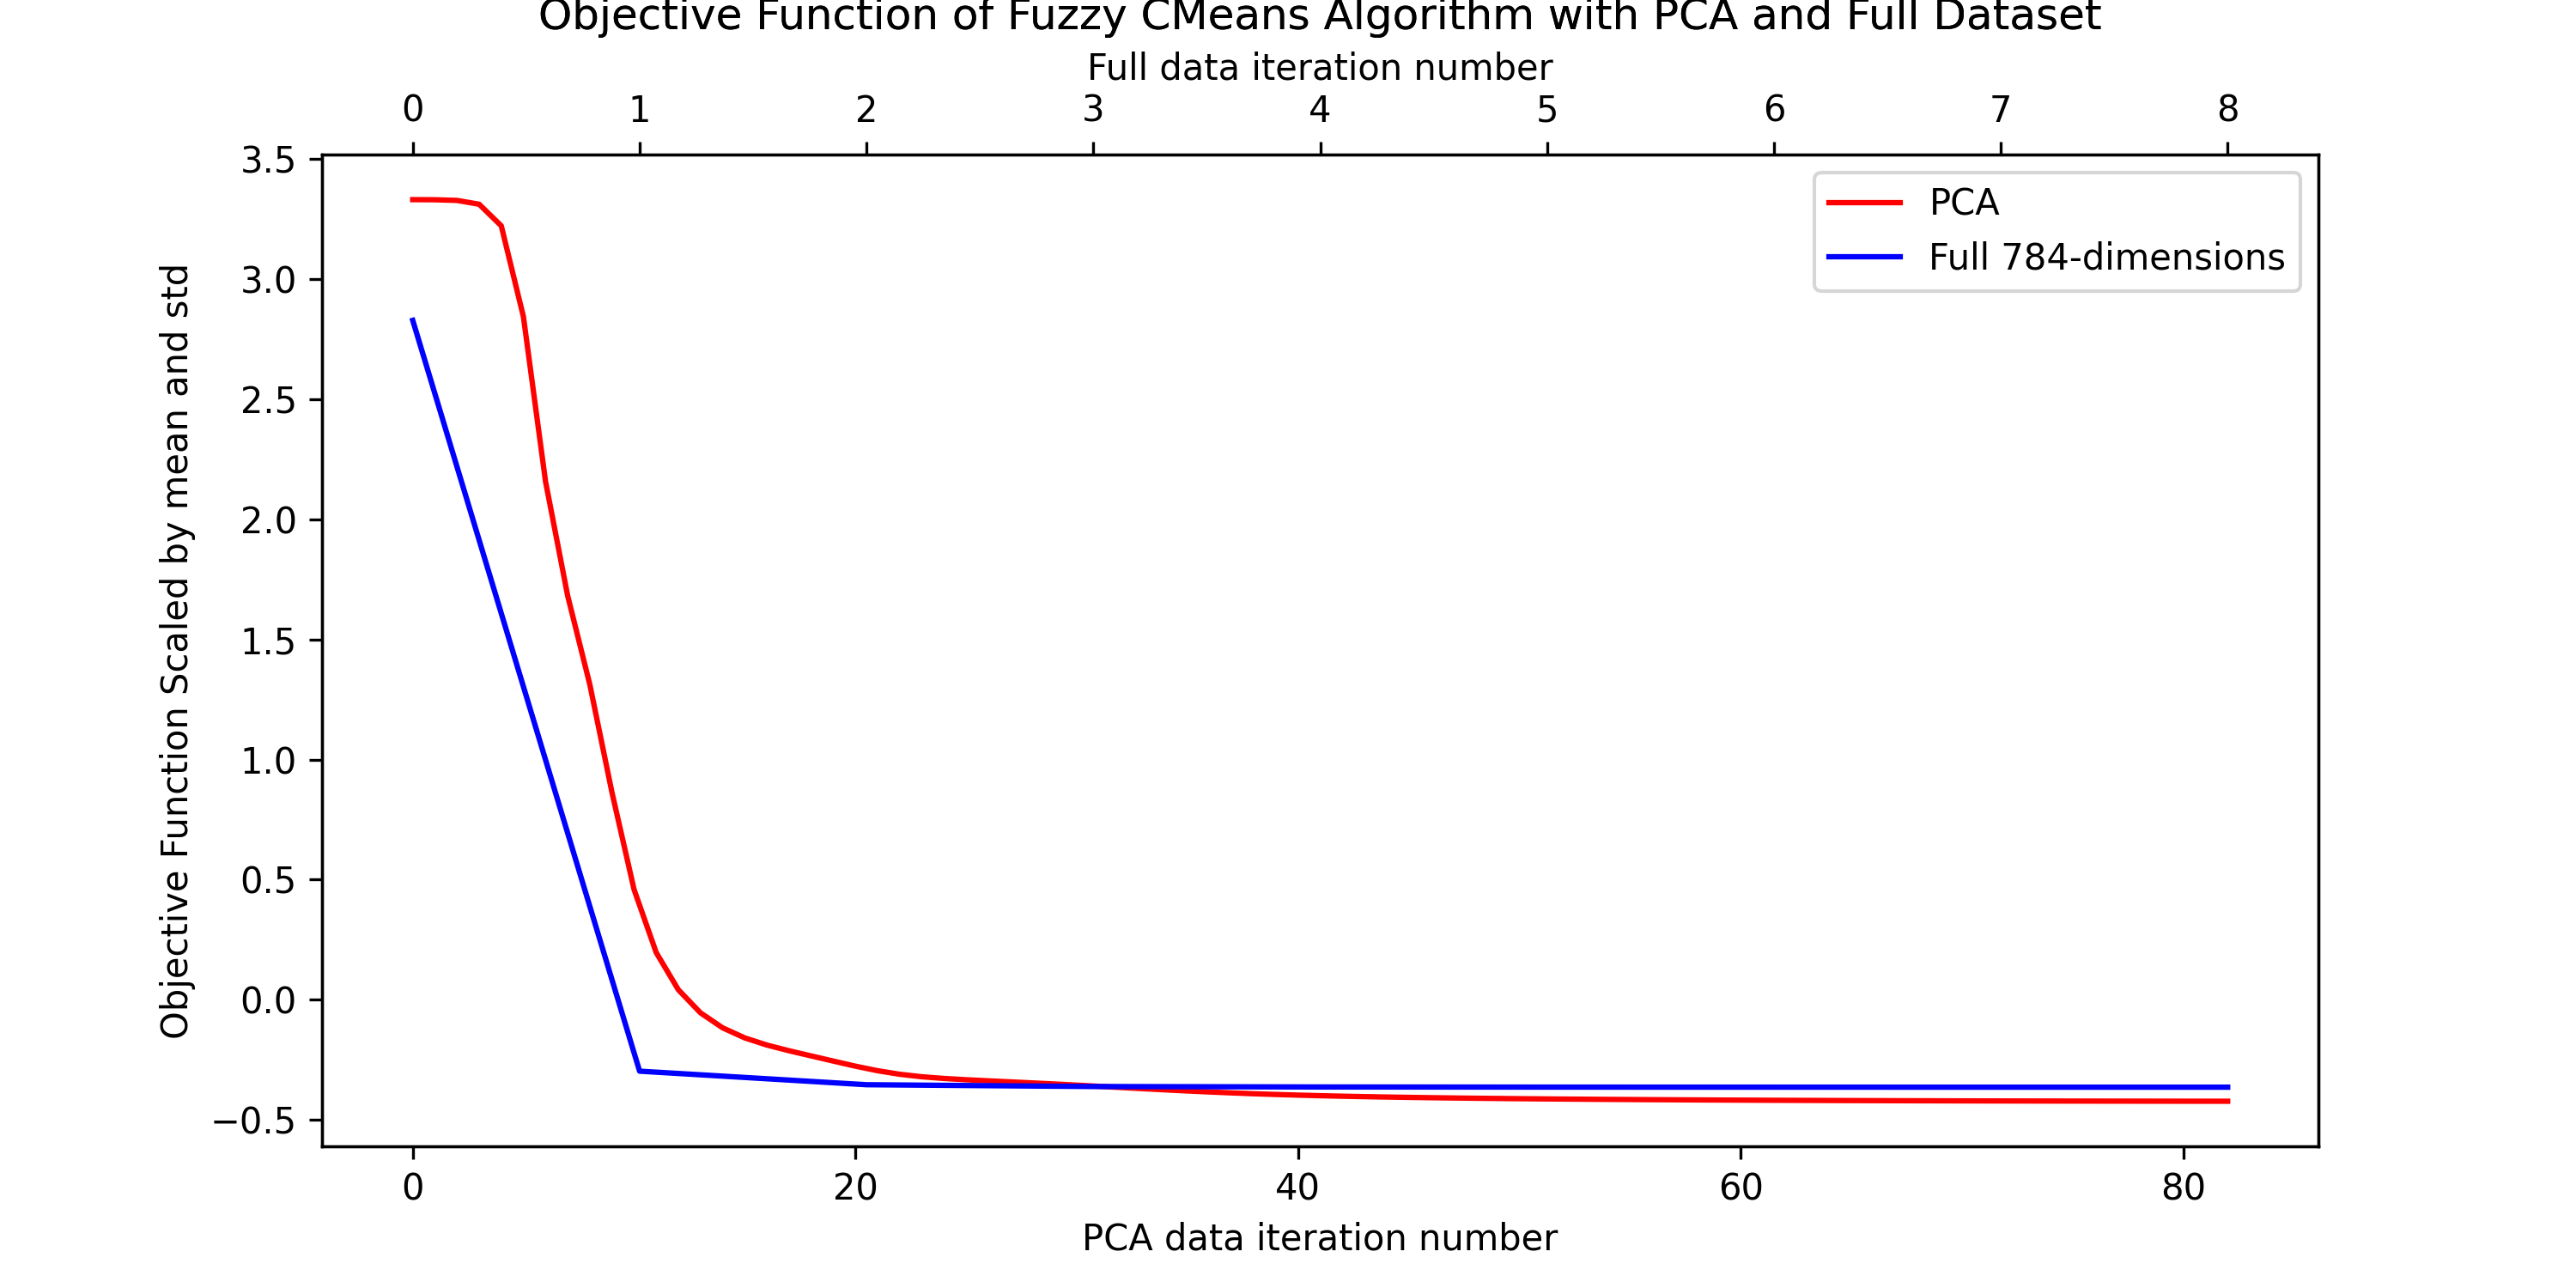
\includegraphics[width=0.5\textwidth]{objective_function_iterations.png}
    \caption{St. Dev. Normalized obejective functions through runtime of the FCM algorithm}
    \label{fig:objective_function_iterations}    
\end{figure}

The RI results for the full data set resulted in a value of 0.692 and the PCA dataset resulted in a value of 0.672.

We also plotted the results of FCM applied to the PCA dataset. The clusters are graphed according by color according to their class label. 
There is also a black X to indicate the cluster center.

\begin{figure}[H]
    \centering
    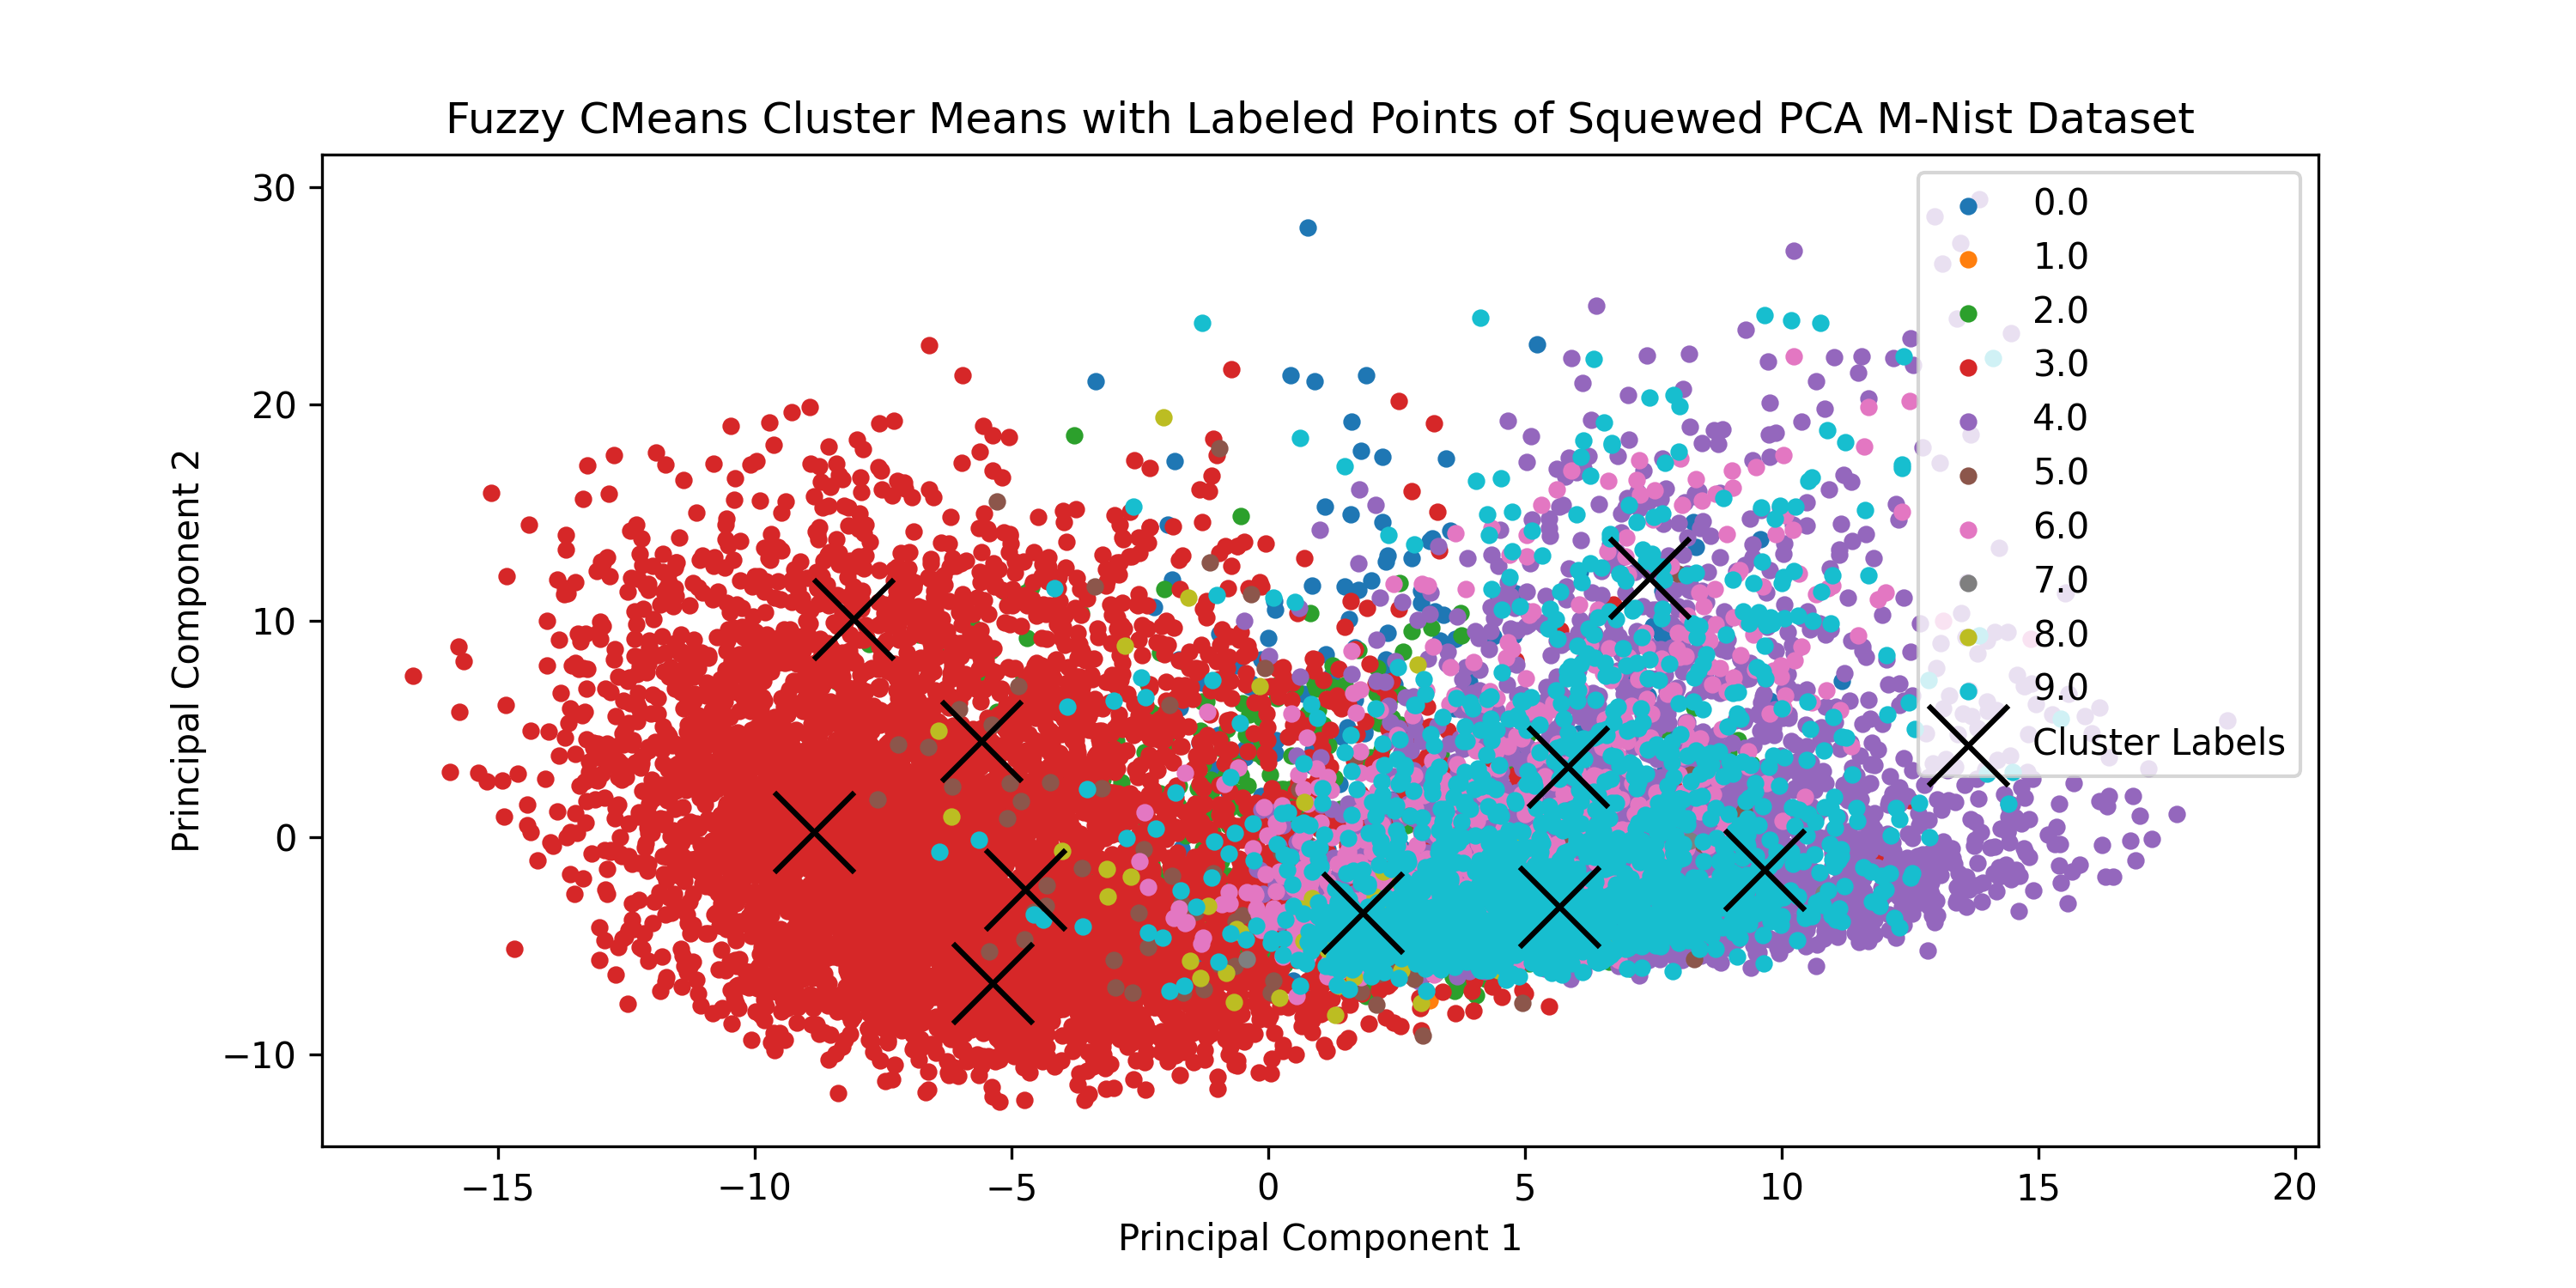
\includegraphics[width=0.5\textwidth]{pca_cluster_means.png}
    \caption{Clusters produced by FCM applied to the PCA dataset}
    \label{fig:pca_clusters}
\end{figure}

\end{multicols}
\begin{figure}[H]
    \centering
    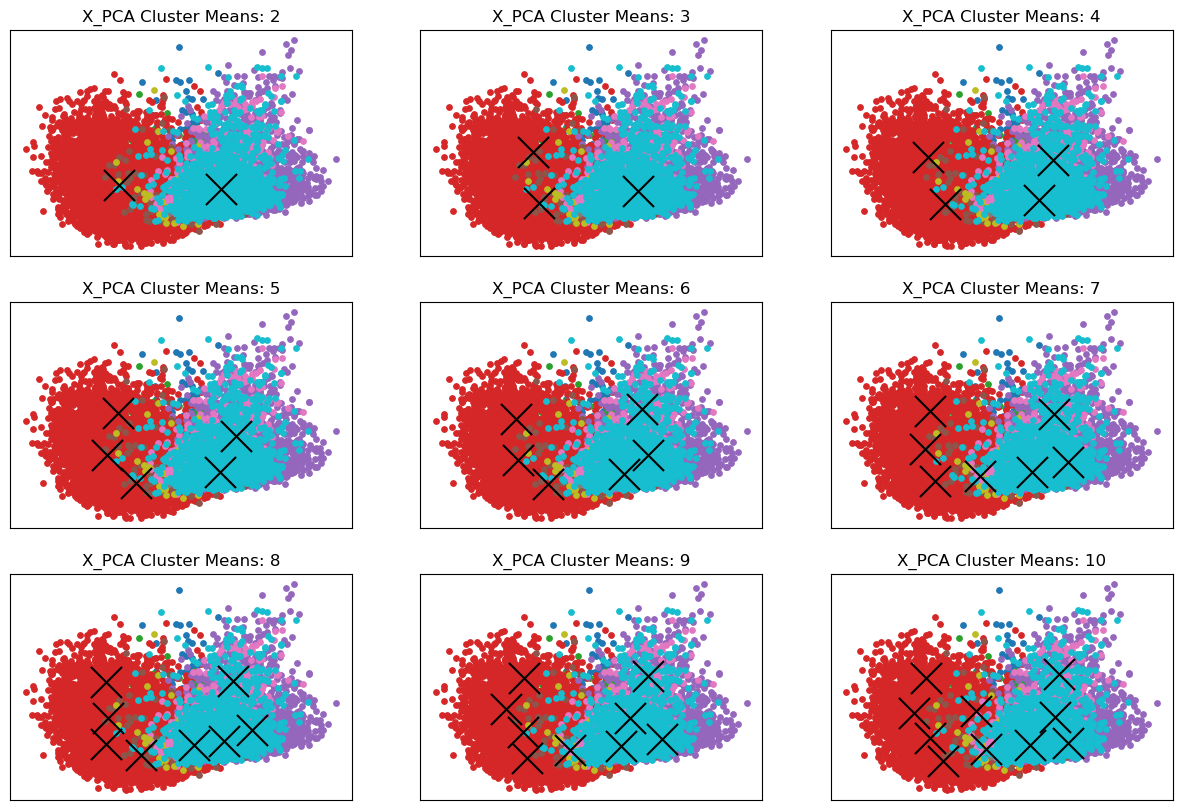
\includegraphics[width=1\textwidth]{X_pca_multiple_cluster_experiment.png}
    \caption{RI results for different cluster amounts applied to the PCA dataset}
    \label{fig:pca_cluster_amounts}
\end{figure}
\begin{multicols}{2}

Additionaly, we wanted to evaluate the PCA dataset with different cluster amounts. We ran the FCM algorithm with cluster amounts of 2, 3, 4, 5, 6, 7, 8, 9, and 10. The results are shown in figure~\ref{fig:pca_cluster_amounts}, and the following table.\newline\newline\newline\newline

\small
\begin{center}    
    Cluster Evaluation for PCA Dataset Table
    \begin{tabular}{ccc}
        %Cluster Evaluation & Metrics for PCA & Dataset \\
        \hline
        Clusters & PCA Rand Index & Scaled All Dim Rand Index \\
        \hline
        2 & 0.6927 & 0.6884 \\
        3 & 0.6799 & 0.6938 \\
        4 & 0.6809 & 0.6922 \\
        5 & 0.6739 & 0.6922 \\
        6 & 0.6766 & 0.6903 \\
        7 & 0.6766 & 0.6917 \\
        8 & 0.6753 & 0.6923 \\
        9 & 0.6726 & 0.6922 \\
        10 & 0.6737 & 0.6713 \\
        \hline
    \end{tabular}        
\end{center}
\normalsize



